\title{BI-EXTENSIONS OF FORMAL GROUPS}
\markright{Bi-Extensions of Formal Groups}

\author{By~~ David Mumford}
\date{}

\maketitle

\setcounter{pageoriginal}{306}
In\pageoriginale the Colloquium itself, I announced that all abelian varieties can be lifted to characteristic zero. The proof of this, as sketched there, is roughly as follows.
\begin{itemize}
\item[(i)] It suffices to prove that every char $p$ abelian variety is a specialization of a char $p$ abelian variety with multiplicative formal group (an ``ordinary'' abelian variety), since Serre (unpublished) has shown that these admit liftings.

\item[(ii)] A preliminary reduction of the problem was made to abelian varieties $X$ such that the invariant
$$
\alpha(X)=\dim_{k}\Hom (\alpha_{p},X)
$$
is $1$.

\item[(iii)] A method was found to construct deformations of a polarized abelian variety from deformations of its polarized Dieudonn\'e module.

\item[(iv)] Finally, some simple deformations of polarized Dieudonn\'e modules were constructed to establish the result.
\end{itemize}

However, it seems premature to give this proof here, since the basic method used in (iii) promises to give much fuller information on the local structure of the formal moduli space of a polarized abelian variety, and this would make my {\em ad hoc} method obsolete. I want instead to give some basic information on the main new technical tool which is used in (iii).

\section{Cartier's result}\label{art15-sec1}

In the note \cite{art15-key1}, Cartier has announced a module-theoretic classification of formal groups over arbitrary ground-rings $R$. We require only the special case where $p=0$ in $R$, which is foreshadowed in Dieudonn'es original paper \cite{art15-key2}, before the category men got a hold of it, modifying the technique until the restriction ``$R$ = perfect field'' came to seem essential.

\begin{defi*}
Let\pageoriginale $R$ be a ring of characteristic $p$. Let $W(R)$ be the ring of Witt vectors over $R$, and let
\begin{align*}
(a_{0},a_{1},a_{2},\ldots)^{\sigma} &= (a^{p}_{0},a^{p}_{1},a^{p}_{2},\ldots),\\[3pt]
(a_{0},a_{1},a_{2},\ldots)^{t} &= (0,a_{0},a_{1},\ldots). 
\end{align*}
Then $A_{R}$ will denote the ring
$$
W(R)[[V]][F]
$$
modulo the relations:
\begin{itemize}
\item[{\rm(a)}] $FV=p$,

\item[{\rm(b)}] $VaF=a^{t}$,

\item[{\rm(c)}] $Fa=a^{\sigma}F$,

\item[{\rm(d)}] $aV=Va^{\sigma}$,
\end{itemize}
for all $a\in W(R)$.
\end{defi*}

\begin{theorem*}[Dieudonn\'e-Cartier]
There is a covariant equivalence of categories between
\begin{itemize}
\item[{\rm(A)}] the category of commutative formal groups $\Phi$ over $R$, and

\item[{\rm(B)}] the category of left $A_{R}$-modules $M$ such that
\begin{itemize}
\item[{\rm(a)}] $\bigcap\limits_{i}V^{i}M=(0)$,

\item[{\rm(b)}] $Vm=0\Rightarrow m=0$, all $m\in M$,

\item[{\rm(c)}] $M/VM$ is a free $R$-module of finite rank.
\end{itemize}
\end{itemize}
\end{theorem*}

The correspondence between these 2 categories can be set up as follows. Recall first that a formal group $\Phi/R$ (by which we mean a set of $n$ power series $\phi_{i}(x_{1},\ldots,x_{n};y_{1},\ldots,y_{n})$, $1\leq i\leq n$, satisfying the usual identities, c.f. Lazard \cite{art15-key3}) defines a covariant functor $F_{\Phi}$ from $R$-algebbras $S$ to groups : i.e. $\forall \ S/R$,
$$
F_{\Phi}(S)=\{(a_{1},\ldots,a_{n})|a_{i}\in S, a_{i}\text{~nilpotent}\}
$$
where
$$
(a_{1},\ldots,a_{n})\cdot (b_{1},\ldots,b_{n})=(\phi_{1}(a_{1},\ldots,a_{n};b_{1},\ldots,b_{n}),\ldots,\phi_{n}(a_{1},\ldots,a_{n};b_{1},\ldots,b_{n})).
$$
N. B. In what follows, we will often call the functor $F_{\Phi}$ instead of the power series $\Phi$ the formal group, for simplicity.

Let\pageoriginale $\widehat{W}$ be the functor
$$
\left\{
\begin{array}{l}
\widehat{\bfW}=\{(a_{0},a_{1},\ldots)|a_{i}\in S, a_{i}\text{~ nilpotent, almost all~ } a_{i}=0\},\\
\text{gp law } = \text{Witt vector addition.}
\end{array}\right.
$$
Then we attach to the commutative formal group $\Phi$ the set
$$
M=\Hom_{\text{gp. functors/}R}(\widehat{R},F_{\Phi}),
$$
and since $A_{R}\cong \Hom (\widehat{\bfW},\widehat{\bfW})^{0}$, we can endow $M$ with the structure of left $A_{R}$-module. Conversely, to go in the other direction, first note that any $A_{R}$-module $M$ as in the theorem can be resolved:
\begin{equation*}
0\to A^{n}_{R}\xrightarrow{\beta}A^{n}_{R}\xrightarrow{\alpha}M\to 0.\tag{*}
\end{equation*}
In fact, choose $m_{1},\ldots,m_{n}\in M$ whose images $\mod VM$ are a basis of $M/VM$ as $R$-module. Define
$$
\alpha(P_{1},\ldots,P_{n})=\sum\limits^{n}_{i=1}P_{i}m_{i}.
$$
It is easy to check that $Fm_{i}$ can be expanded in the form $\sum\limits^{n}_{j=1}Q_{ij}(V)m_{j}$, $Q_{ij}$ a power series in $V$ with coefficients in $W(R)$. Define
$$
\beta(P_{1},\ldots,P_{n})=\left(\sum\limits^{n}_{i=1}P_{i}\cdot Q_{i1}-\delta_{i1}F,\ldots,\sum\limits^{n}_{i=1}P_{i}\cdot Q_{in}-\delta_{in}F\right).
$$
It is not hard to check that (*) is exact. Then $\beta$ defines a monomorphism of group functors $\beta^{*}:(\widehat{W})^{n}\to (\widehat{W})^{n}$, and let $F$ be the quotient functor $(\widehat{W})^{n}/\beta^{*}(\widehat{W})^{n}$. Then $F$ is isomorphic to $F_{\Phi}$ for one and-up to canonical isomorphism-only one formal group $\Phi$.

Moreover, we get a resolution of the functor $F_{\Phi}$:
$$
0\to (\widehat{W})^{n}\xrightarrow{\beta^{*}}(\widehat{W})^{n}\to F_{\Phi}\to 0.
$$
When $R$ is a perfect field, the above correspondence can be extended to an analogous correspondence between $p$-divisible groups over $R$ and $W(R)[F,V]$-modules of suitable type (c.f. \cite{art15-key4}, \cite{art15-key5}). However,\pageoriginale it does not seem likely at present that such an extension exists for non-perfect $R$'s. This is a key point.

\section{Bi-extensions of abelian groups}\label{art15-sec2}

Let $A$, $B$, $C$ be 3 abelian groups. $A$ bi-extension of $B\times C$ by $A$ will denote a set $G$ on which $A$ acts freely, together with a map
$$
G\xrightarrow{\pi} B\times C
$$
making $B\times C$ into the quotient $G/A$, together with 2 laws of composition:
\[
\xymatrix@R=.01cm{
+_{1}:\fprod{G}{G}{B}\to G\ar@{=}[ddddd]_-{\text{def}} & ;\quad +_{2}:\fprod{G}{G}{C}\to G\ar@{=}[ddddd]_-{\text{def}}\\
 & & \\
 & & \\
 & & \\
 & & \\
\{(g_{1},g_{2})|\pi(g_{1}),\pi(g_{2})\text{~have}  & \{(g_{1},g_{2})|\pi(g_{1}),\pi(g_{2})\text{~have}\\
\text{same $B$-component}\} & \text{some $C$-component}\}
}
\]
These are subject to the requirement:
\begin{itemize}
\item[(i)] for all $b\in B$, $G'_{b}=\pi^{-1}(b\times C)$ is an abelian group under $+_{1}$, $\pi$ is a surjective homomorphism of $G'_{b}$ onto $C$, and via the action of $A$ on $G'_{b}$, $A$ is isomorphic to the kernel of $\pi$;

\item[(ii)] for all $c\in C$, $G^{2}_{c}=\pi^{-1}(B\times c)$ is an abelian group under $+_{2}$, $\pi$ is a surjective homomorphism of $G^{2}_{c}$ onto $B$, and via the action of $A$ on $G^{2}_{c}$, $A$ is isomorphic to the kernel of $\pi$;

\item[(iii)] given $x$, $y$, $u$, $v\in G$ such that
\begin{align*}
\pi(x) &= (b_{1},c_{1})\\
\pi(y) &= (b_{1},c_{2})\\
\pi(u) &= (b_{2},c_{1})\\
\pi(v) &= (b_{2},c_{2}),
\end{align*}
then 
$$
(x+_{1}y)+_{2}(u+_{1}v)=(x+_{2}u)+_{1}(y+_{2}v).
$$
This\pageoriginale may seem like rather a mess, but please consider the motivating example: let $X$ be an abelian variety over an algebraically closed field $k$, let $\widehat{X}$ be its dual, and let $P$ be the universal, or Poincar\'e, line bundle on over $X\times \widehat{X}$. Then $P_{k}$, the underlying set of closed points of $P$, is a bi-extension of $X_{k}\times \widehat{X}_{k}$ by $k^{*}$!
\end{itemize}

Notice that if $G$ is a bi-extension of $B\times C$ by $A$, then $\pi^{-1}(B\times 0)$ splits canonically into $A\times B$, and $\pi^{-1}(0\times C)$ splits canonically into $A\times C$. In fact, we can lift $B$ to $\pi^{-1}(B\times 0)$ by mapping $b\in B$ to the element of $G$ which is the identity in $\pi^{-1}(b\times C)$; and we can lift $C$ to $\pi^{-1}(0\times C)$ by mapping $c\in C$ to the element of $G$ which is the identity in $\pi^{-1}(B\times c)$.

Bi-extensions can be conveniently described by co-cycles: choose a (set-theoretic) section
\begin{figure}[H]
\centering
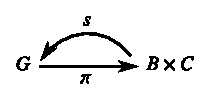
\includegraphics{figures/fig1.eps}
\end{figure}
Via $s$ and the action of $A$ on $G$, we construct an isomorphism
$$
G\cong A\times B\times C
$$
such that the action of $A$ on $G$ corresponds to the action of $A$ on $A\times B\times C$ which is just addition of $A$-components, leaving the $B$-and $C$-components fixed. Then $+_{1}$ and $+_{2}$ go over into laws of composition on $A\times B\times C$ given by:
\begin{align*}
& (a,b,c)+_{1}(a',b,c')=(a+a'+\phi(b;c,c'),b,c+c')\\
& (a,b,c)+_{2}(a',b',c)=(a+a'+\psi (b,b';c),b+b',c).
\end{align*}
For $+_{1}$, $+_{2}$ to be abelian group laws, we need:
\begin{itemize}
\item[(a)] $\phi(b;c+c',c'')+\phi(b;c,c')=\phi(b;c,c'+c'')+\phi(b;c',c'')$

\centerline{$\phi(b;c,c')=\phi(b;c',c);$}

\item[(b)] $\psi(b+b',b'';c)+\psi(b,b';c)=\psi(b,b'+b'';c)+\psi(b',b'';c)$

\centerline{$\psi(b,b';c)=\psi(b',b;c)$.}
\smallskip


The final restriction comes out as:
\item[(c)] $\phi(b+b';c,c')-\phi(b;c,c')-\phi(b';c,c')$\pageoriginale

$=\psi(b,b';c+c')-\psi(b,b';c)-\psi(b,b';c')$.
\end{itemize}
What are the co-boundaries? If you alter $s$ by adding to it a map $\rho:B\times C\to A$, then you check that the new $\phi'$, $\psi'$ are related to the old ones by
\begin{align*}
&\phi'(b;c,c')-\phi(b;c,c')=\rho(b,c+c')-\rho(b,c)-\rho(b,c')\\
&\psi'(b,b';c)-\psi(b,b';c)=\rho(b+b',c)-\rho(b,c)-\rho(b,c).
\end{align*}

Using this explicit expression by co-cycles and co-boundaries, it is clear that the set of all bi-extensions of $B\times C$ by $A$ forms itself an abelian group, which we will denote
$$
\text{Bi-ext~}(B\times C,A).
$$

It is also clear, either from the definition or via co-cycles, that Bi-ext is a covariant functor in $A$, and a contravariant functor in $B$ and $C$.

\section{Bi-extensions of group-functors}\label{art15-sec3}

\begin{defi*}
If $F$, $G$, $H$ are $3$ covariant functors from the category of $R$-algebras to the category of abelian groups, a bi-extension of $G\times H$ by $F$ is a fourth functor $K$ such that for every $R$-algebra $S$, $K(S)$ is a bi-extension of $G(S)\times H(S)$ by $F(S)$ and for every $R$-homomorphism $S_{1}\to S_{2}$, the map $K(S_{1})\to K(S_{2})$ is a homomorphism of bi-extensions (in the obvious sense). In particular, if $F$, $G$, $H$ are formal groups, this gives us a bi-extension of formal groups.
\end{defi*}

If $F$, $G$, $H$ are formal groups, it is easy again to compute the bi-extensions $K$ by power series co-cycles. In fact, one merely has to check that:
\begin{itemize}
\item[(i)] there is a functorial section
\begin{figure}[H]
\centering
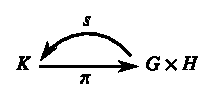
\includegraphics{figures/fig2.eps}
\end{figure}
(this\pageoriginale % 313
\end{itemize}
